\documentclass[11pt]{article}
\usepackage[margin=0.8in]{geometry}
\usepackage[utf8]{inputenc}
\usepackage{graphicx}
\usepackage{booktabs}
\usepackage{array}
\usepackage{multirow}
\usepackage{amsmath}
\usepackage{placeins}
\usepackage[font=small,skip=6pt]{caption}
\usepackage{subcaption}
\usepackage{microtype}
\usepackage{url}
\usepackage{iftex}
\ifXeTeX
  % XeTeX (tectonic): OpenType Times/Helvetica clones, matching main.tex
  \usepackage{fontspec}
  \setmainfont{texgyretermes}[Extension=.otf, UprightFont=*-regular, BoldFont=*-bold,
    ItalicFont=*-italic, BoldItalicFont=*-bolditalic]
  \setsansfont{texgyreheros}[Extension=.otf, UprightFont=*-regular, BoldFont=*-bold,
    ItalicFont=*-italic, BoldItalicFont=*-bolditalic]
\else
  \usepackage{mathptmx}
\fi
\urlstyle{same}
\captionsetup{labelfont=bf,justification=centering}
\renewcommand{\arraystretch}{1.08}
\setlength{\parskip}{6pt}
\setlength{\parindent}{0pt}
\renewcommand{\thetable}{S\arabic{table}}
\renewcommand{\thefigure}{S\arabic{figure}}
\renewcommand{\topfraction}{0.95}
\renewcommand{\textfraction}{0.05}
\renewcommand{\floatpagefraction}{0.8}
% Item numbers follow the reviewer's mapping table (Table M1), so each float sets its own
% number; numbers that the mapping does not assign are left unused.
\newcommand{\tablenumber}[1]{\setcounter{table}{\numexpr#1-1\relax}}
\newcommand{\figurenumber}[1]{\setcounter{figure}{\numexpr#1-1\relax}}
\newcommand{\panel}[3]{\begin{subfigure}[t]{#1\linewidth}\centering\includegraphics[width=\linewidth]{#2}\caption{#3}\end{subfigure}}

\begin{document}

\begin{center}
{\Large\bfseries Supplementary Material}\\[6pt]
{\large Standardised Comparison of Convolutional and Transformer Backbones for Brain Tumour MRI Classification under Perceptual-Hash Deduplication}\\[6pt]
Parth Mital, Ved Lawand, Biji C. L., Muzaffar Ahamad Dar, George Priya Doss C.
\end{center}

This document accompanies the main manuscript. Item numbers are those cited in the main text. Unless stated otherwise, every quantity is measured on the held-out test split, which was evaluated once per model using the checkpoint selected on the validation split. The per-model artefacts from which every table and figure here was produced are released with the code repository described in the main manuscript.

\section*{S1. Dataset characterisation}

Figures~S1 and S2 show the native image dimension and intensity distributions of the two experimental tracks, summarised numerically in Table~3 of the main text. Figure~S3 shows the class distribution of the binary detection dataset, and Figure~S4 the stratified training, validation, and test split distributions of both tracks, whose per-class counts are given in Table~4 of the main text.

\begin{figure}[htbp]
\figurenumber{1}
\centering
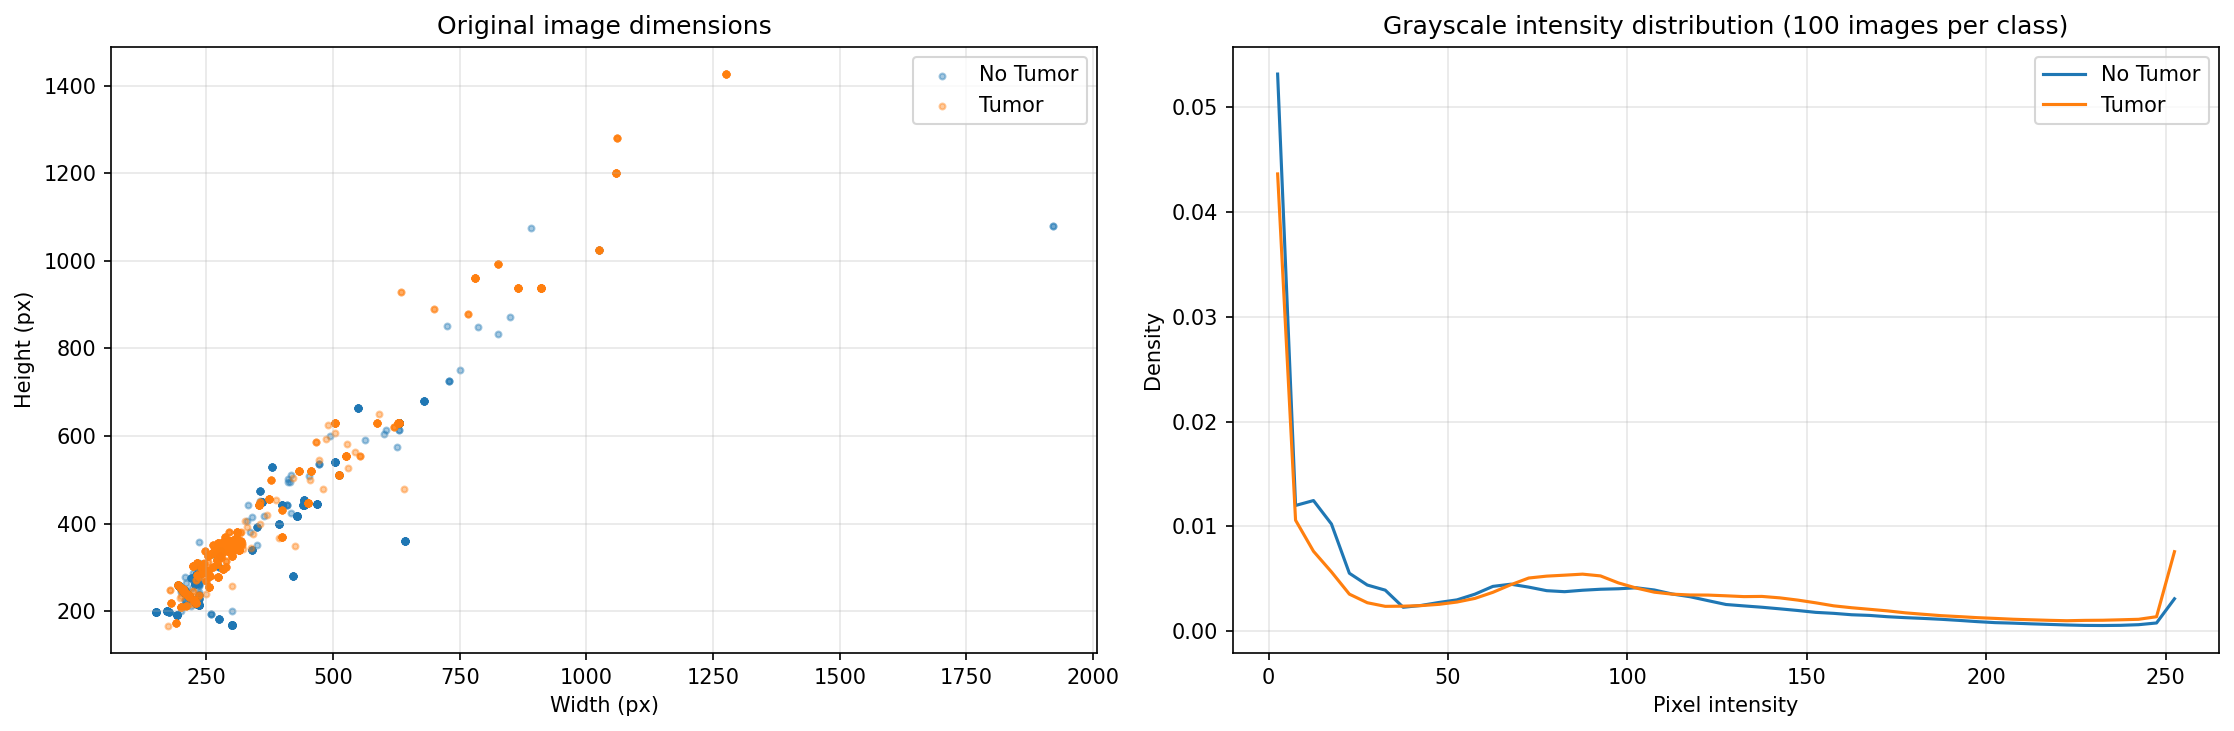
\includegraphics[width=\linewidth]{figures/binary_image_properties.png}
\caption{Native image dimension and intensity distributions for the binary detection dataset, showing the wide variation in resolution and field of view across the two contributing sources.}
\label{fig:s1}
\end{figure}

\begin{figure}[htbp]
\figurenumber{2}
\centering
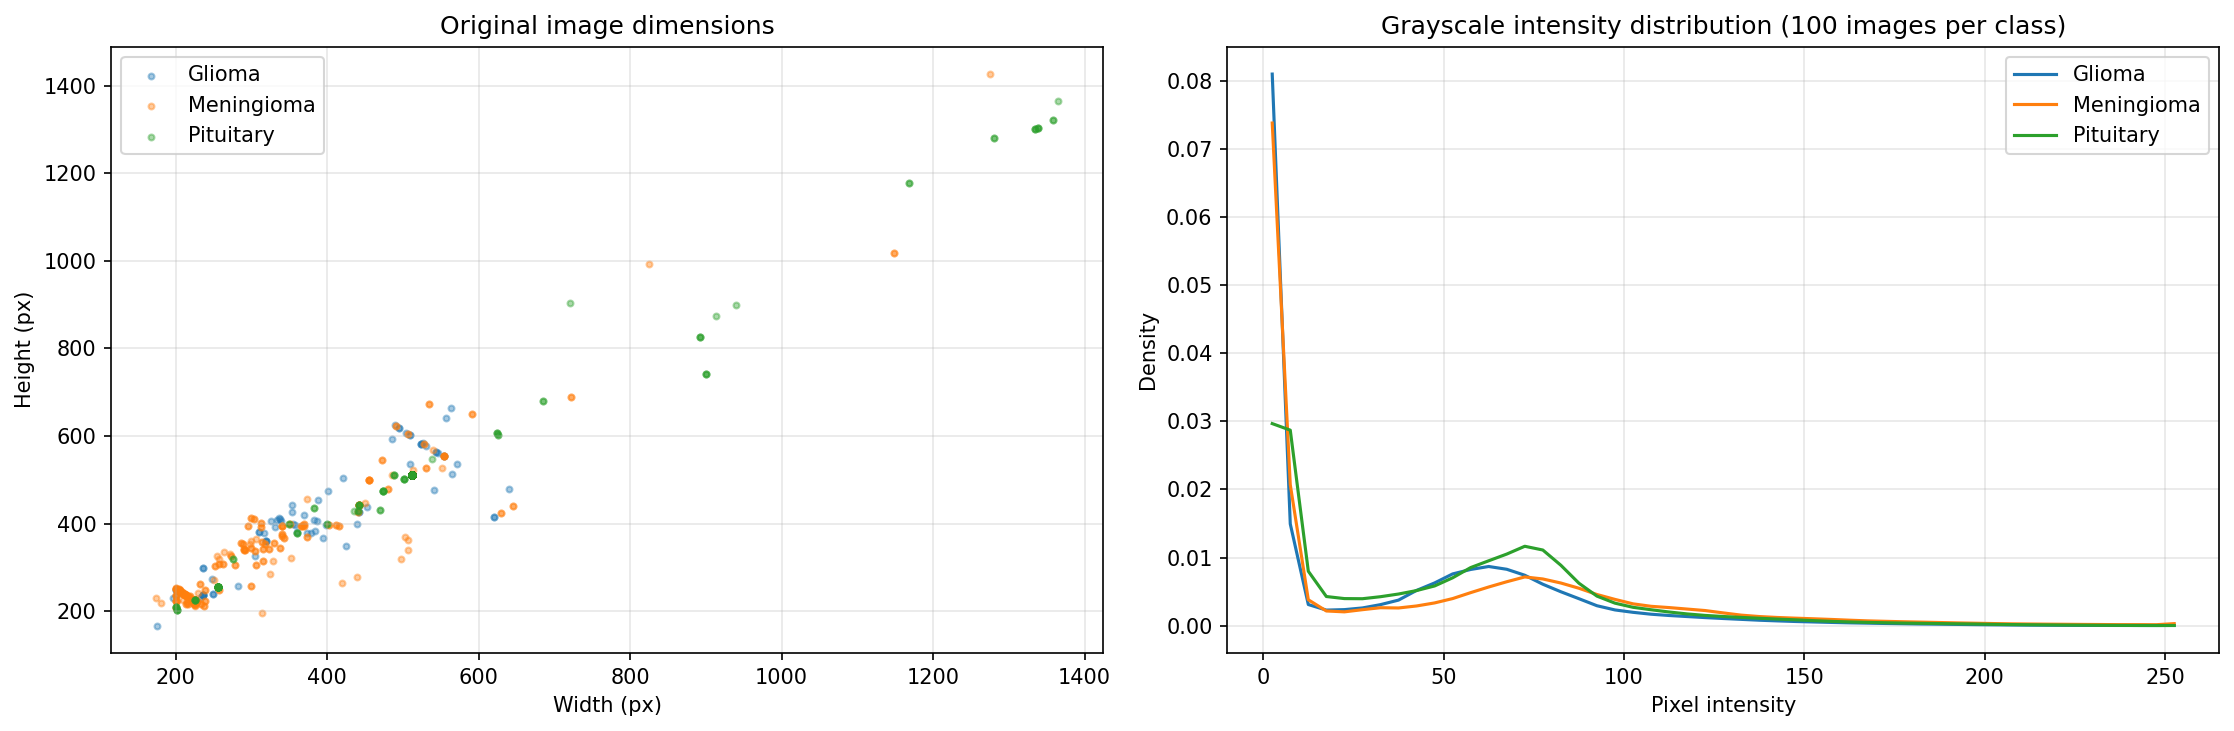
\includegraphics[width=\linewidth]{figures/cls_image_properties.png}
\caption{Native image dimension and intensity distributions for the multiclass classification dataset before deduplication, which is markedly more homogeneous than the binary collection, with a median resolution of $512\times 512$ pixels in every class.}
\label{fig:s2}
\end{figure}

\begin{figure}[htbp]
\figurenumber{3}
\centering
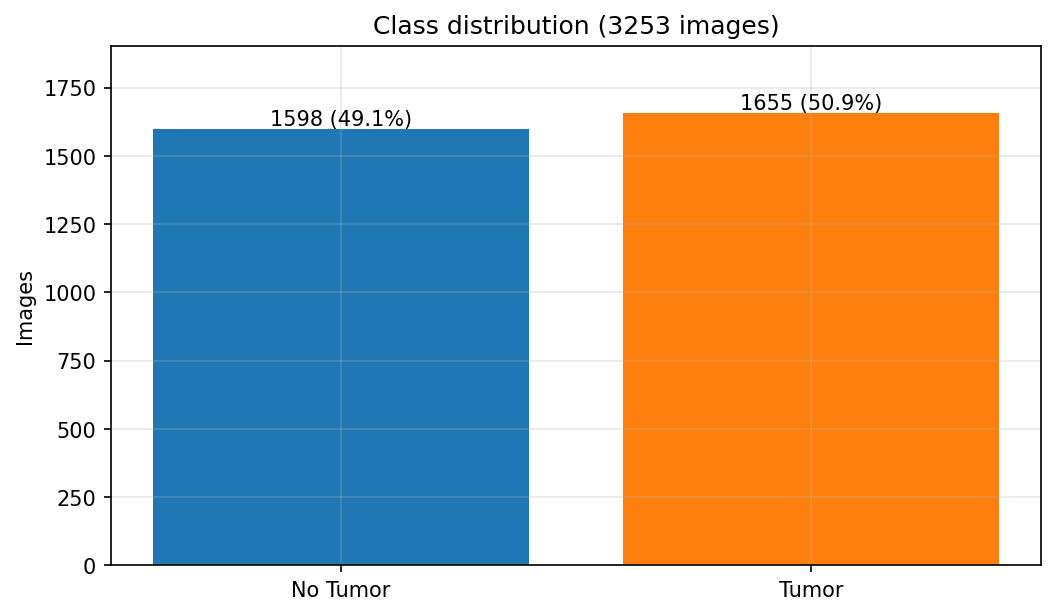
\includegraphics[width=0.6\linewidth]{figures/binary_class_distribution.png}
\caption{Class distribution of the combined binary detection dataset, comprising 1,598 tumour-negative and 1,655 tumour-positive images.}
\label{fig:s3}
\end{figure}

\begin{figure}[htbp]
\figurenumber{4}
\centering
\panel{1}{figures/binary_split.png}{Binary detection.}
\\[4pt]
\panel{1}{figures/cls_split.png}{Multiclass classification, after deduplication.}
\caption{Stratified training, validation, and test split distributions for both tasks, in the proportions 70\%, 15\%, and 15\%.}
\label{fig:s4}
\end{figure}

The remaining items of this section come from a post-training audit that reproduced the original data collection, perceptual-hash pass, and stratified splits exactly, without retraining any model. The reproduced multiclass pass retains the published 2,000, 1,304, and 1,401 images per class, and the reproduced splits match the stored test and validation predictions of all 15 runs. Table~S11 gives the per-source survival of both pools, the binary figures being those of a pass that was not applied before training. Figure~S17 plots the native image size of every source. Figure~S18 shows the closest cross-label near-duplicate pairs of the multiclass pool, and Figure~S19 compares the hash with an independent detector based on the normalised cross-correlation (NCC) of $64\times 64$ greyscale thumbnails, which treats a pair as the same image at $\mathrm{NCC}\geq 0.98$. Figure~S20 gives, for every test image, the Hamming distance to its nearest training image, and Table~S12 and Figure~S21 the test accuracy of every model on the test images with no training image within a given distance.

\begin{table}[htbp]
\tablenumber{11}
\centering
\caption{Images per source and class before and after the perceptual-hash pass at a Hamming tolerance of 5. The binary pass was run after training and was not applied to the training data. Of the 1,123 multiclass removals, 3 are cross-source and 1,120 within-source, and 23 are cross-label; of the 2,066 binary removals, 731 are cross-source (Br35H images whose retained near-duplicate is a Chakrabarty image) and none is cross-label.}
\label{tab:s11}
\small
\begin{tabular*}{\textwidth}{@{\extracolsep{\fill}}lllccc@{}}
\toprule
Track & Source & Class & Before & Kept & Removed (\%) \\
\midrule
\multirow{4}{*}{Binary} & Chakrabarty & Tumour-negative & 98 & 76 & 22.45 \\
 & Chakrabarty & Tumour & 155 & 130 & 16.13 \\
 & Br35H & Tumour-negative & 1,500 & 383 & 74.47 \\
 & Br35H & Tumour & 1,500 & 598 & 60.13 \\
\midrule
\multirow{9}{*}{Multiclass} & Bhuvaji, training & Glioma & 826 & 695 & 15.86 \\
 & Bhuvaji, training & Meningioma & 822 & 604 & 26.52 \\
 & Bhuvaji, training & Pituitary & 827 & 626 & 24.30 \\
 & Bhuvaji, testing & Glioma & 100 & 82 & 18.00 \\
 & Bhuvaji, testing & Meningioma & 115 & 98 & 14.78 \\
 & Bhuvaji, testing & Pituitary & 74 & 32 & 56.76 \\
 & Cheng & Glioma & 1,426 & 1,223 & 14.24 \\
 & Cheng & Meningioma & 708 & 602 & 14.97 \\
 & Cheng & Pituitary & 930 & 743 & 20.11 \\
\bottomrule
\end{tabular*}
\end{table}

\begin{table}[htbp]
\tablenumber{12}
\centering
\caption{Test accuracy (\%) of every model on the full test split and on the test images with no training image within Hamming distance 5 or 8, or with no training image at $\mathrm{NCC}\geq 0.98$; the number of test images in each subset is given in the Images rows. Multiclass test images have no training image within distance 5 by construction.}
\label{tab:s12}
\small
\begin{tabular*}{\textwidth}{@{\extracolsep{\fill}}llcccc@{}}
\toprule
Task & Model & Full & Distance $>5$ & Distance $>8$ & No NCC duplicate \\
\midrule
\multirow{10}{*}{Binary} & Images & 488 & 85 & 47 & 92 \\
\cmidrule(l){2-6}
 & CoAtNet-0 & 99.39 & 98.82 & 97.87 & 98.91 \\
 & DenseNet121 & 99.39 & 97.65 & 95.74 & 97.83 \\
 & EfficientNetB0 & 99.39 & 96.47 & 93.62 & 96.74 \\
 & ResNet50 & 99.39 & 96.47 & 93.62 & 96.74 \\
 & InceptionV3 & 98.77 & 95.29 & 91.49 & 95.65 \\
 & Swin-Base & 95.90 & 89.41 & 89.36 & 90.22 \\
 & ViT-B/16 & 94.88 & 91.76 & 89.36 & 92.39 \\
 & MobileNetV3-Large & 90.78 & 80.00 & 74.47 & 80.43 \\
 & VGG16 & 88.32 & 82.35 & 72.34 & 79.35 \\
\midrule
\multirow{7}{*}{Multiclass} & Images & 706 & 706 & 265 & 703 \\
\cmidrule(l){2-6}
 & Swin-Base & 98.58 & 98.58 & 97.74 & 98.58 \\
 & CoAtNet-0 & 98.44 & 98.44 & 97.36 & 98.44 \\
 & InceptionV3 & 98.30 & 98.30 & 98.11 & 98.29 \\
 & EfficientNetB0 & 97.59 & 97.59 & 96.23 & 97.58 \\
 & ResNet50 & 97.59 & 97.59 & 96.98 & 97.58 \\
 & ViT-B/16 & 90.51 & 90.51 & 90.19 & 90.47 \\
\bottomrule
\end{tabular*}
\end{table}

\begin{figure}[htbp]
\figurenumber{17}
\centering
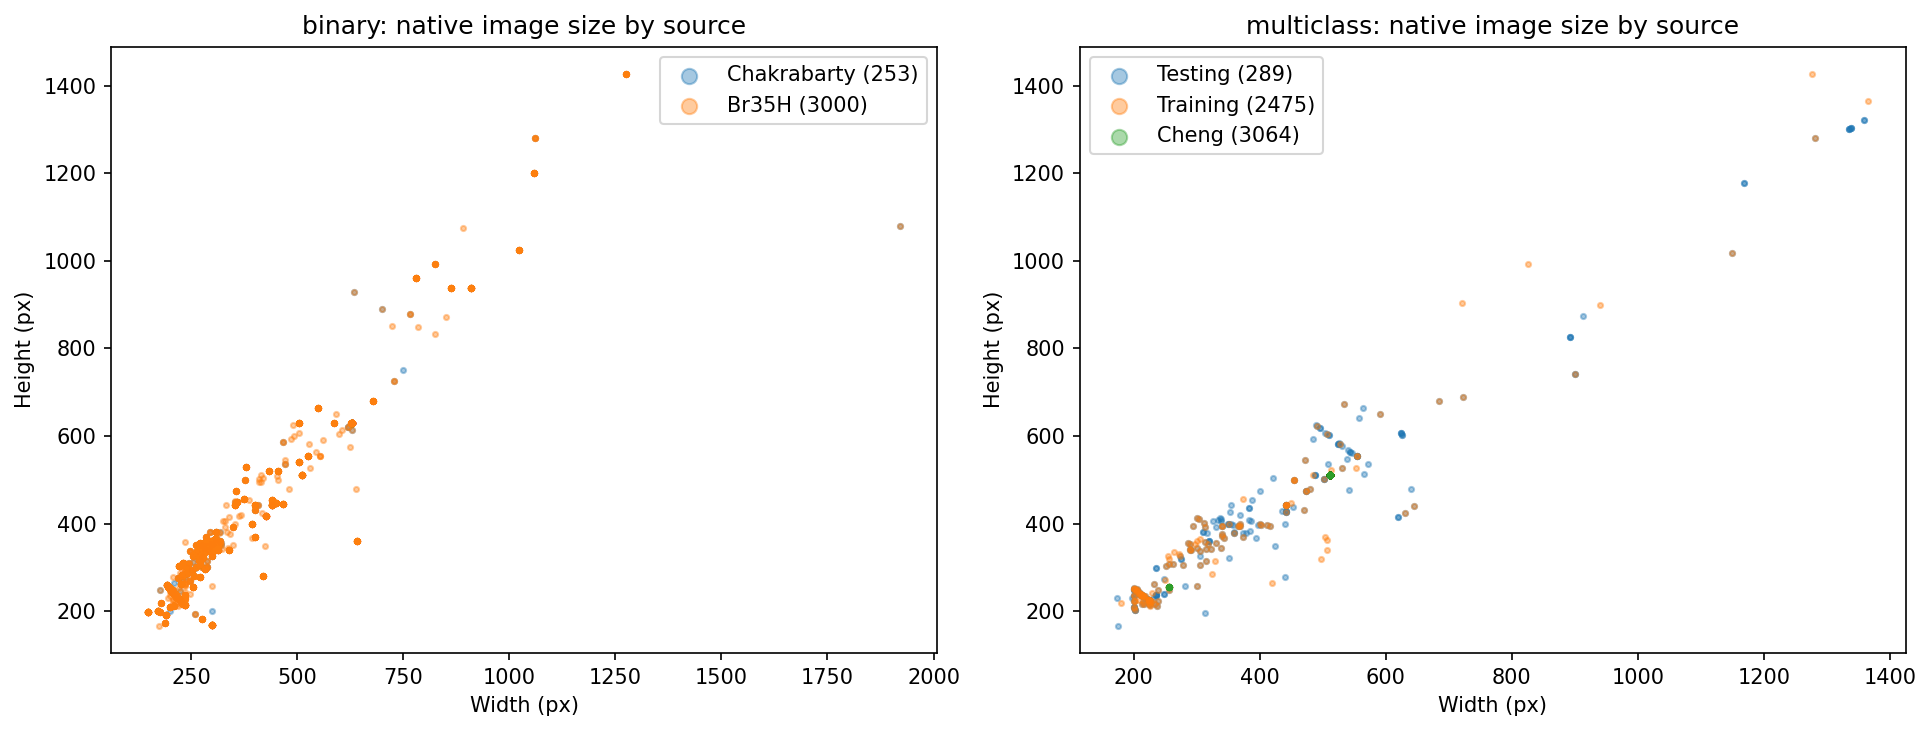
\includegraphics[width=\linewidth]{figures/audit/01_native_size_by_source.png}
\caption{Native width and height of every image by source, for the binary pool (left) and the multiclass pool (right), where the Bhuvaji collection is split into its original training and testing folders. Almost all Cheng slices and most Bhuvaji training images are $512\times 512$ pixels, whereas the Bhuvaji testing folder and both binary sources span a wide range of sizes.}
\label{fig:s17}
\end{figure}

\begin{figure}[htbp]
\figurenumber{18}
\centering
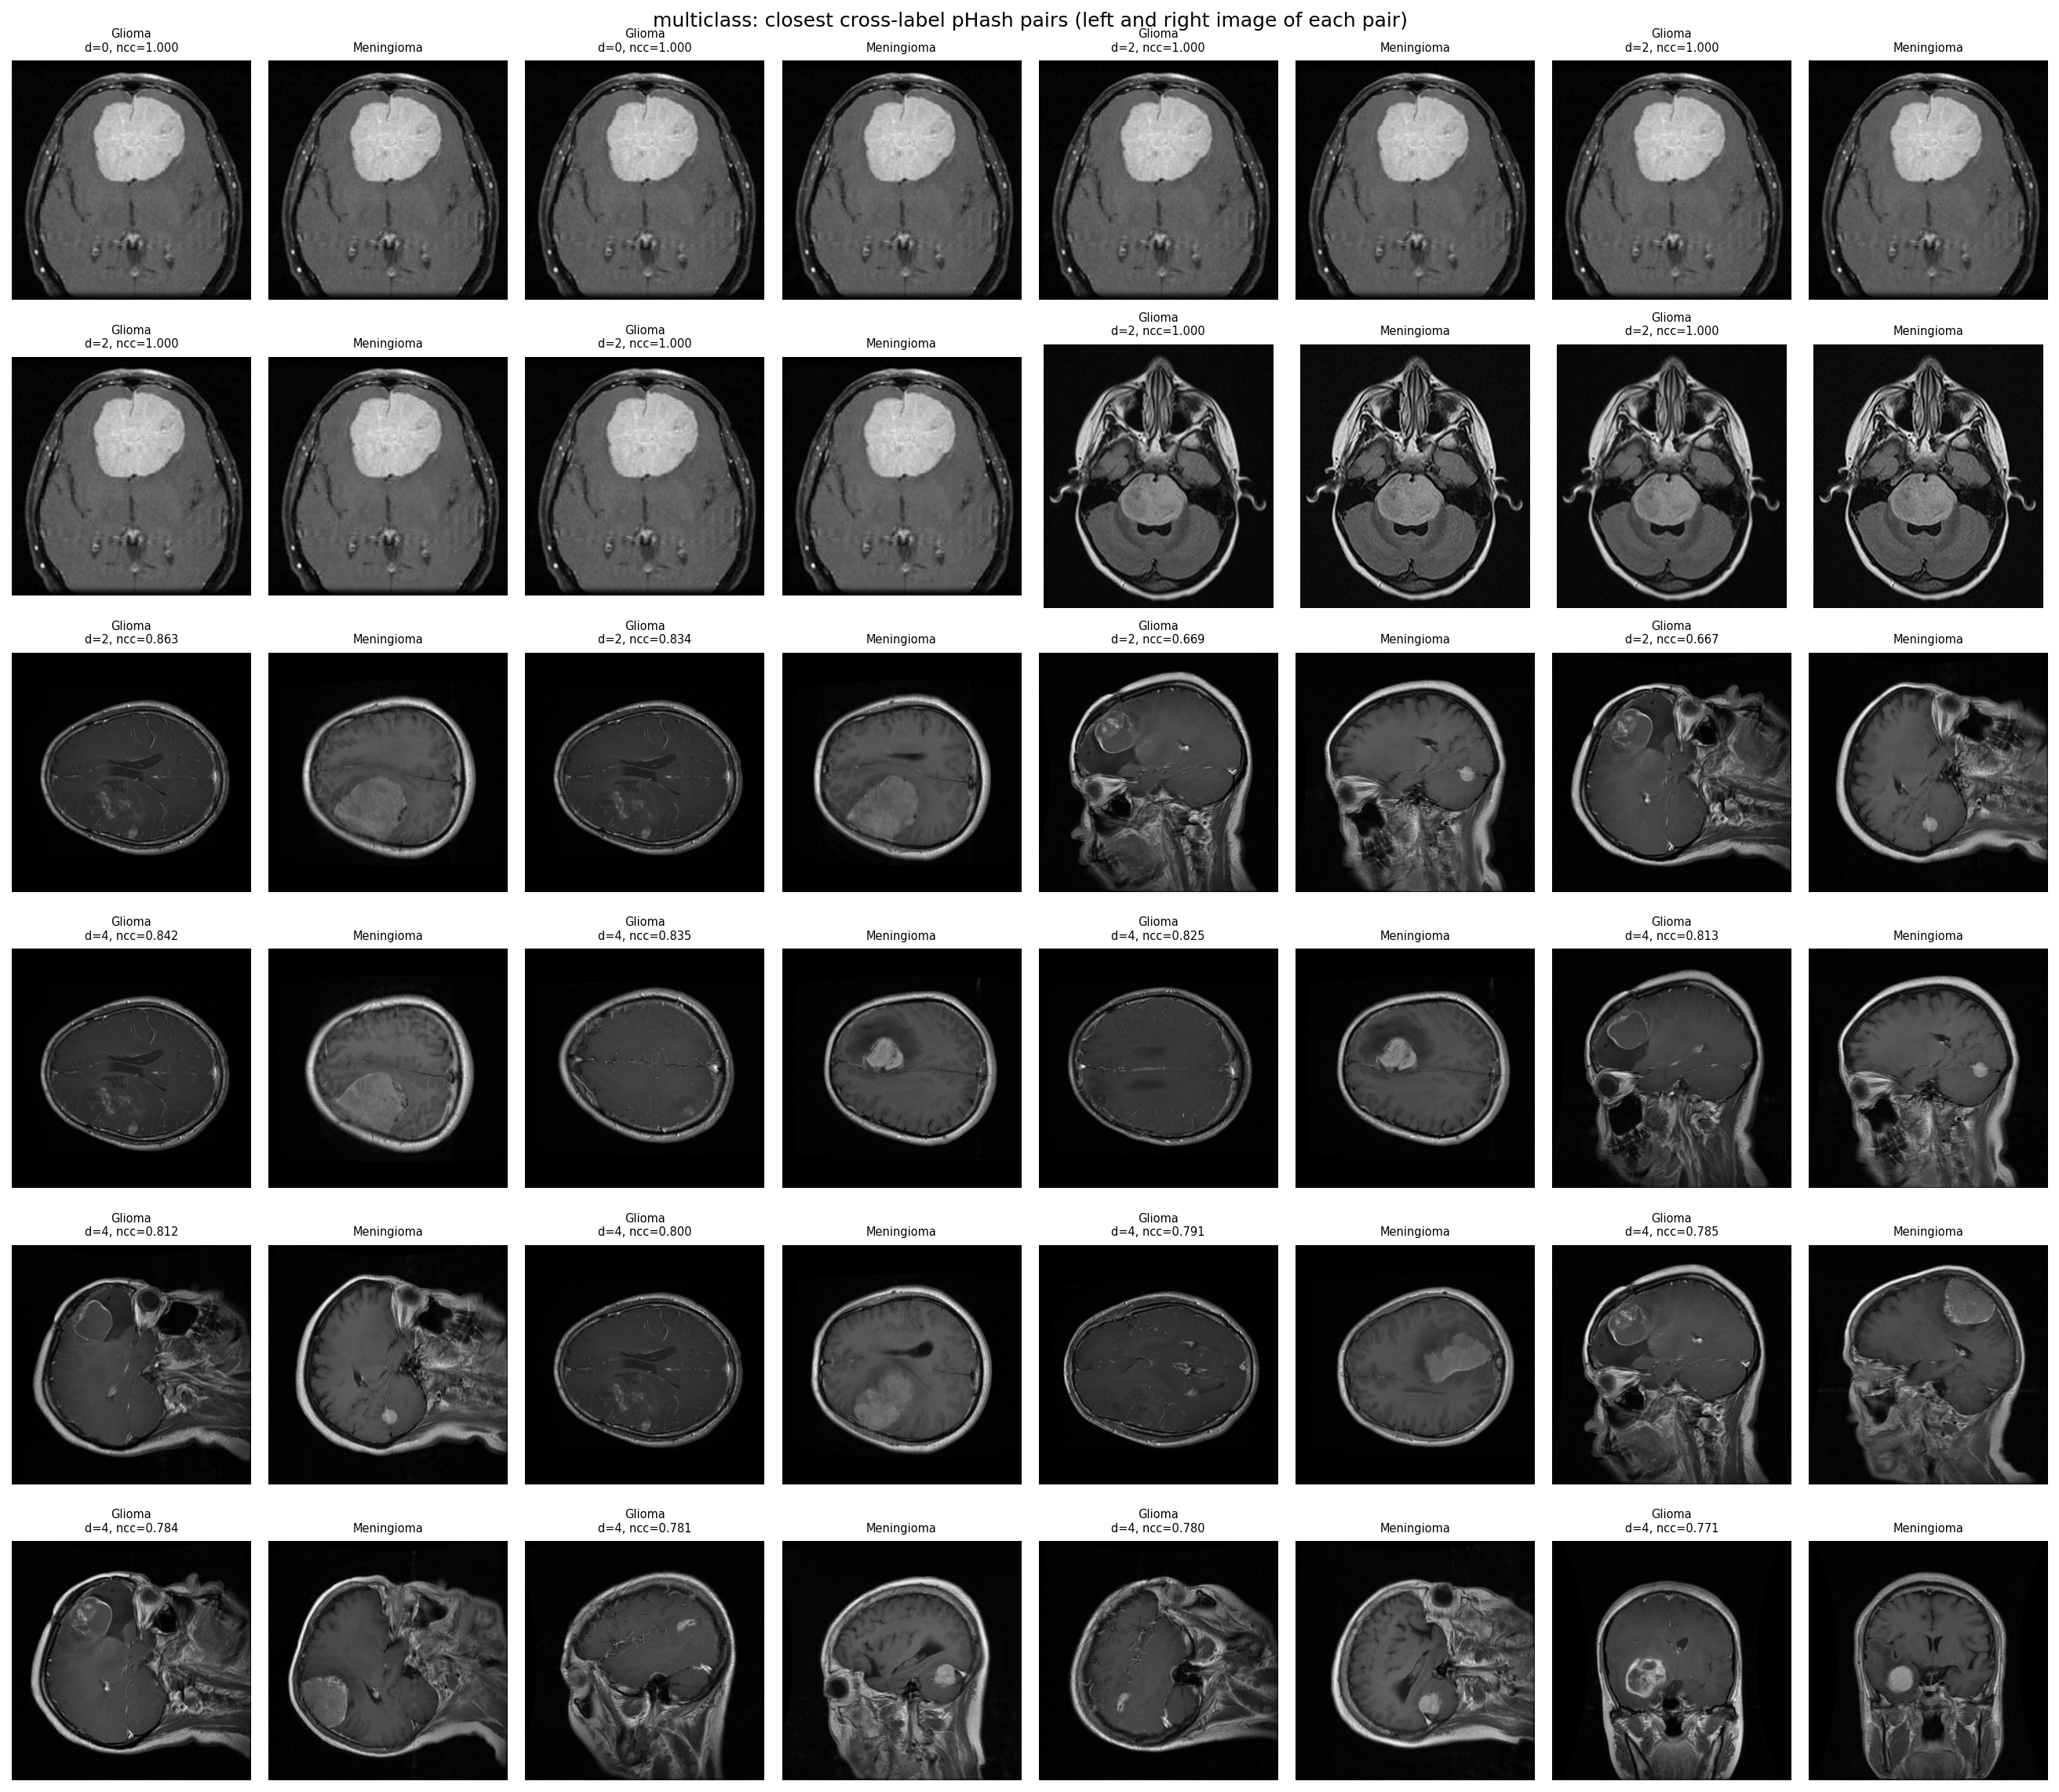
\includegraphics[width=\linewidth]{figures/audit/02_multiclass_cross_label_gallery.png}
\caption{The closest cross-label near-duplicate pairs of the multiclass pool, each shown as a glioma image beside a meningioma image with their Hamming distance $d$ and thumbnail NCC. All 31 cross-label pairs within the tolerance are glioma against meningioma. The 8 pairs at $\mathrm{NCC}\geq 0.98$ are the same images filed under both labels in the Bhuvaji collection; the other 23 are visually distinct images and are hash false positives.}
\label{fig:s18}
\end{figure}

\begin{figure}[htbp]
\figurenumber{19}
\centering
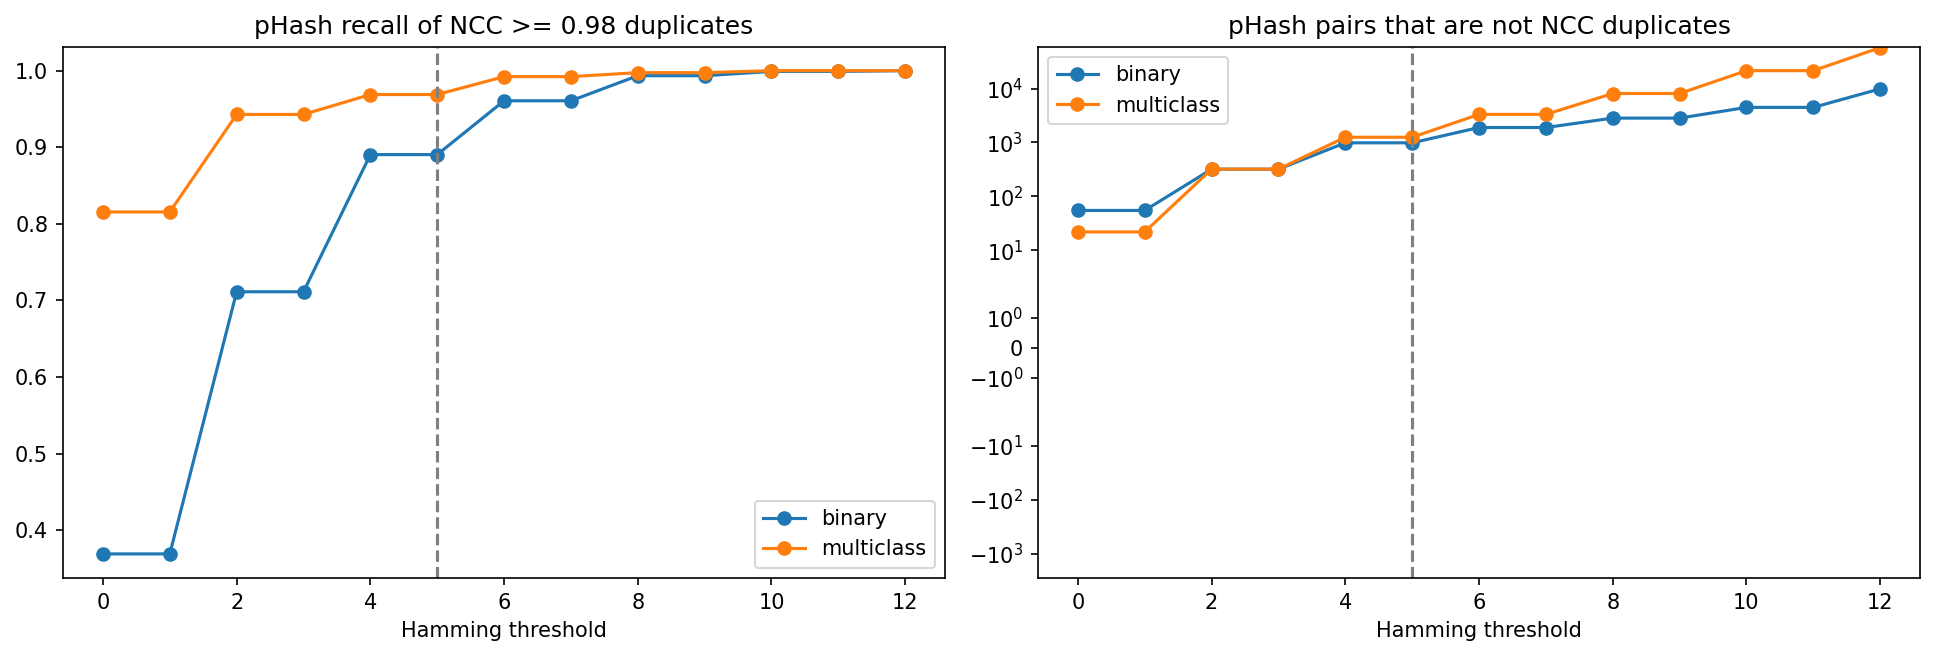
\includegraphics[width=\linewidth]{figures/audit/03_phash_vs_ncc.png}
\caption{Perceptual hash against the NCC detector as a function of the Hamming tolerance. Left: share of NCC duplicate pairs (385 multiclass, 6,078 binary) that the hash also flags. Right: number of hash pairs that are not NCC duplicates, on a logarithmic scale. At the tolerance of 5 used in this study (dashed line) the hash recovers 96.9\% and 89.0\% of the NCC pairs and flags 1,250 and 986 further pairs.}
\label{fig:s19}
\end{figure}

\begin{figure}[htbp]
\figurenumber{20}
\centering
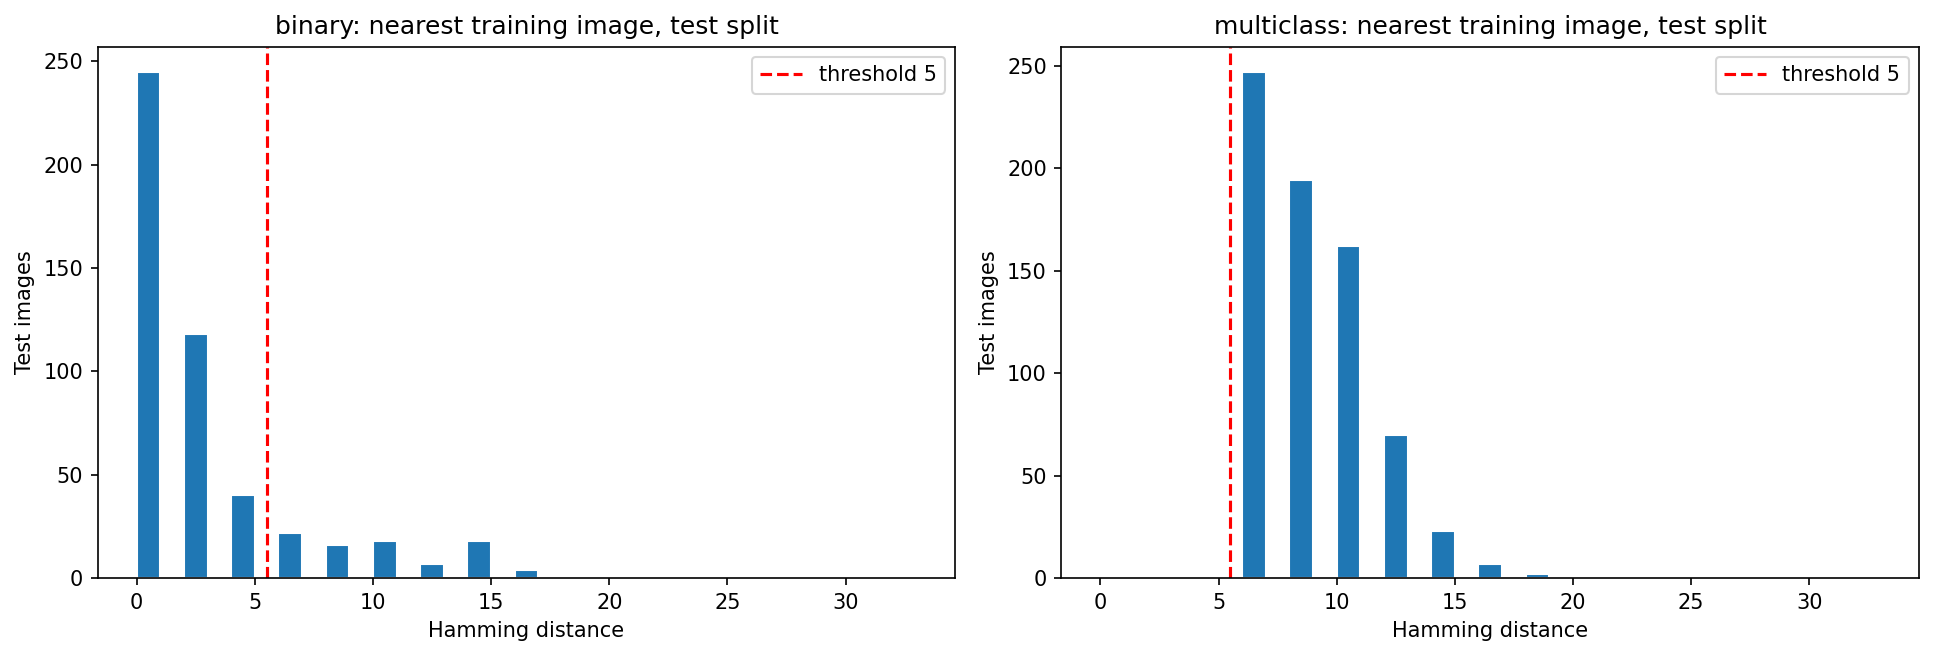
\includegraphics[width=\linewidth]{figures/audit/04_train_test_nearest_distance.png}
\caption{Hamming distance from every test image to its nearest training image. In the binary track, which was not deduplicated, 403 of 488 test images (82.6\%) lie within the tolerance of 5. In the multiclass track no test image does, by construction.}
\label{fig:s20}
\end{figure}

\begin{figure}[htbp]
\figurenumber{21}
\centering
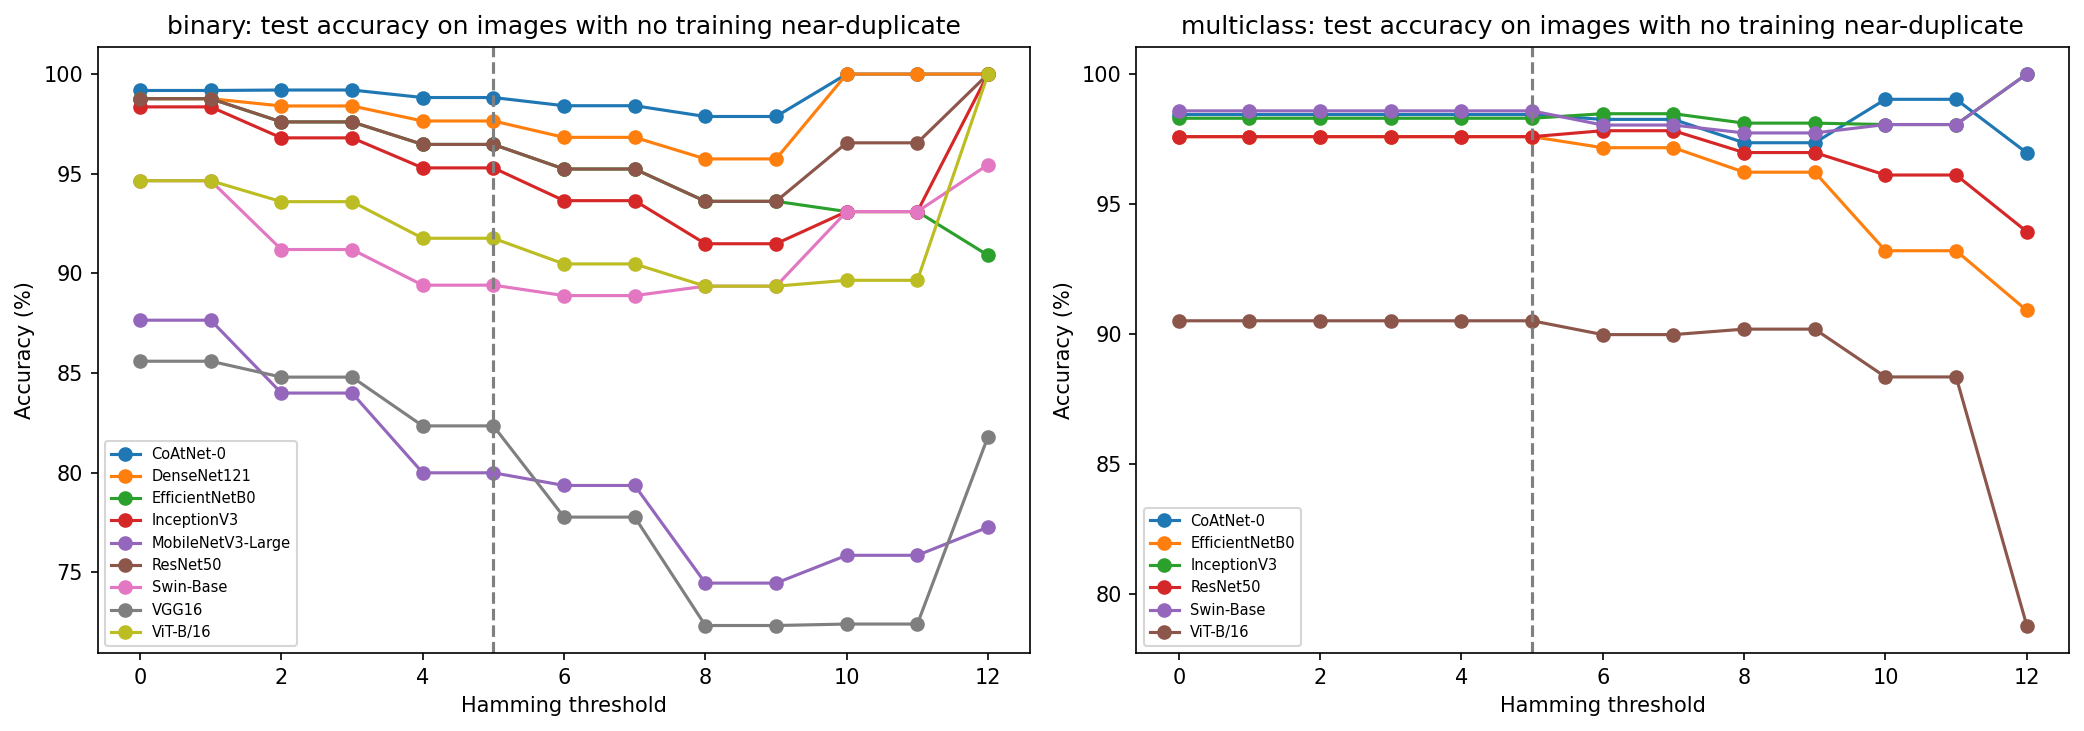
\includegraphics[width=\linewidth]{figures/audit/05_accuracy_by_threshold.png}
\caption{Test accuracy of every model on the test images with no training image within each Hamming distance, computed from the stored test predictions without retraining. The subsets shrink as the distance grows (Table~S12), to 22 binary and 33 multiclass images at a distance of 12, so the right-hand end of each curve rests on very few images.}
\label{fig:s21}
\end{figure}

\FloatBarrier
\section*{S3. Preprocessing and augmentation}

\begin{figure}[htbp]
\figurenumber{6}
\centering
\panel{1}{figures/binary_augmentation.png}{Binary detection task.}
\\[4pt]
\panel{1}{figures/cls_augmentation.png}{Multiclass classification task.}
\caption{Representative MRI images before and after the training-time augmentation pipeline, comprising random horizontal flipping, random rotation of up to $\pm 10$ degrees, and brightness and contrast jitter of up to 20\%.}
\label{fig:s6}
\end{figure}

\FloatBarrier
\section*{S4. Per-class metrics}

Tables~S4 and S5 give the per-class precision, sensitivity, specificity, and F1 score of every model on the held-out test split. Support is the number of test images in each class.

\begin{table}[htbp]
\tablenumber{4}
\centering
\caption{Per-class binary detection metrics on the held-out test split.}
\label{tab:s4}
\small
\begin{tabular*}{\textwidth}{@{\extracolsep{\fill}}llccccc@{}}
\toprule
Model & Class & Support & Prec. (\%) & Sens. (\%) & Spec. (\%) & F1 (\%) \\
\midrule
CoAtNet-0 & No tumour & 240 & 100.00 & 98.75 & 100.00 & 99.37 \\
 & Tumour & 248 & 98.80 & 100.00 & 98.75 & 99.40 \\
\midrule
DenseNet121 & No tumour & 240 & 98.77 & 100.00 & 98.79 & 99.38 \\
 & Tumour & 248 & 100.00 & 98.79 & 100.00 & 99.39 \\
\midrule
EfficientNetB0 & No tumour & 240 & 100.00 & 98.75 & 100.00 & 99.37 \\
 & Tumour & 248 & 98.80 & 100.00 & 98.75 & 99.40 \\
\midrule
ResNet50 & No tumour & 240 & 98.77 & 100.00 & 98.79 & 99.38 \\
 & Tumour & 248 & 100.00 & 98.79 & 100.00 & 99.39 \\
\midrule
InceptionV3 & No tumour & 240 & 97.95 & 99.58 & 97.98 & 98.76 \\
 & Tumour & 248 & 99.59 & 97.98 & 99.58 & 98.78 \\
\midrule
Swin-Base & No tumour & 240 & 93.65 & 98.33 & 93.55 & 95.93 \\
 & Tumour & 248 & 98.31 & 93.55 & 98.33 & 95.87 \\
\midrule
ViT-B/16 & No tumour & 240 & 96.14 & 93.33 & 96.37 & 94.71 \\
 & Tumour & 248 & 93.73 & 96.37 & 93.33 & 95.03 \\
\midrule
MobileNetV3-Large & No tumour & 240 & 84.21 & 100.00 & 81.85 & 91.43 \\
 & Tumour & 248 & 100.00 & 81.85 & 100.00 & 90.02 \\
\midrule
VGG16 & No tumour & 240 & 86.45 & 90.42 & 86.29 & 88.39 \\
 & Tumour & 248 & 90.30 & 86.29 & 90.42 & 88.25 \\
\bottomrule
\end{tabular*}
\end{table}

\begin{table}[htbp]
\tablenumber{5}
\centering
\caption{Per-class multiclass classification metrics on the held-out test split.}
\label{tab:s5}
\small
\begin{tabular*}{\textwidth}{@{\extracolsep{\fill}}llccccc@{}}
\toprule
Model & Class & Support & Prec. (\%) & Sens. (\%) & Spec. (\%) & F1 (\%) \\
\midrule
Swin-Base & Glioma & 300 & 99.00 & 99.33 & 99.26 & 99.17 \\
 & Meningioma & 196 & 98.95 & 95.92 & 99.61 & 97.41 \\
 & Pituitary & 210 & 97.67 & 100.00 & 98.99 & 98.82 \\
\midrule
CoAtNet-0 & Glioma & 300 & 98.03 & 99.67 & 98.52 & 98.84 \\
 & Meningioma & 196 & 98.43 & 95.92 & 99.41 & 97.16 \\
 & Pituitary & 210 & 99.05 & 99.05 & 99.60 & 99.05 \\
\midrule
InceptionV3 & Glioma & 300 & 98.99 & 98.33 & 99.26 & 98.66 \\
 & Meningioma & 196 & 96.00 & 97.96 & 98.43 & 96.97 \\
 & Pituitary & 210 & 99.52 & 98.57 & 99.80 & 99.04 \\
\midrule
EfficientNetB0 & Glioma & 300 & 98.66 & 98.00 & 99.01 & 98.33 \\
 & Meningioma & 196 & 95.92 & 95.92 & 98.43 & 95.92 \\
 & Pituitary & 210 & 97.64 & 98.57 & 98.99 & 98.10 \\
\midrule
ResNet50 & Glioma & 300 & 98.99 & 97.67 & 99.26 & 98.32 \\
 & Meningioma & 196 & 94.53 & 96.94 & 97.84 & 95.72 \\
 & Pituitary & 210 & 98.56 & 98.10 & 99.40 & 98.33 \\
\midrule
ViT-B/16 & Glioma & 300 & 91.28 & 90.67 & 93.60 & 90.97 \\
 & Meningioma & 196 & 83.50 & 85.20 & 93.53 & 84.34 \\
 & Pituitary & 210 & 96.15 & 95.24 & 98.39 & 95.69 \\
\bottomrule
\end{tabular*}
\end{table}

\FloatBarrier
\section*{S5. Training dynamics}

Table~S6 reports the training and validation metrics at the best epoch for each model on the binary detection task, where the best epoch is the one giving the highest validation AUC. Table~S7 reports the same quantities for the multiclass task at the checkpointed epoch, the one giving the highest validation macro one-versus-rest AUC. Because this metric saturates near 0.997, it distinguishes only weakly between late epochs, and for several models validation accuracy continued to rise after the checkpointed epoch; Swin-Base, for example, is checkpointed at epoch 7 with a validation accuracy of 97.31\%, although its validation accuracy reaches 98.16\% at epochs 9 and 10. These are validation-split figures; the corresponding test-split results are given in Tables~7 and 8 of the main text. Figures~S7 and S8 show the training and validation curves of every model.

\begin{table}[htbp]
\tablenumber{6}
\centering
\caption{Binary detection training and validation metrics at the best epoch, selected by validation AUC.}
\label{tab:s6}
\small
\begin{tabular*}{\textwidth}{@{\extracolsep{\fill}}lccccccc@{}}
\toprule
Model & Epoch & Train loss & Train acc. & Train AUC & Val. loss & Val. acc. & Val. AUC \\
\midrule
CoAtNet-0 & 6 & 0.0114 & 0.9969 & 0.9999 & 0.0322 & 0.9898 & 0.9999 \\
DenseNet121 & 4 & 0.0099 & 0.9969 & 1.0000 & 0.0042 & 1.0000 & 1.0000 \\
EfficientNetB0 & 4 & 0.0307 & 0.9937 & 0.9996 & 0.0178 & 0.9959 & 0.9999 \\
ResNet50 & 7 & 0.0042 & 0.9990 & 1.0000 & 0.0184 & 0.9939 & 0.9999 \\
InceptionV3 & 3 & 0.0314 & 0.9922 & 0.9997 & 0.0106 & 0.9959 & 1.0000 \\
Swin-Base & 6 & 0.0953 & 0.9665 & 0.9938 & 0.0928 & 0.9693 & 0.9973 \\
ViT-B/16 & 10 & 0.1649 & 0.9439 & 0.9837 & 0.1449 & 0.9406 & 0.9899 \\
MobileNetV3-Large & 10 & 0.0023 & 0.9990 & 1.0000 & 0.3995 & 0.8811 & 0.9993 \\
VGG16 & 10 & 0.2590 & 0.8872 & 0.9603 & 0.2421 & 0.8975 & 0.9687 \\
\bottomrule
\end{tabular*}
\end{table}

\begin{table}[htbp]
\tablenumber{7}
\centering
\caption{Multiclass classification training and validation metrics at the checkpointed epoch, selected by validation macro one-versus-rest AUC.}
\label{tab:s7}
\small
\begin{tabular*}{\textwidth}{@{\extracolsep{\fill}}lccccccc@{}}
\toprule
Model & Epoch & Train loss & Train acc. & Train AUC & Val. loss & Val. acc. & Val. AUC \\
\midrule
Swin-Base & 7 & 0.0333 & 0.9884 & 0.9996 & 0.0861 & 0.9731 & 0.9974 \\
CoAtNet-0 & 9 & 0.0246 & 0.9928 & 0.9998 & 0.1019 & 0.9660 & 0.9975 \\
InceptionV3 & 8 & 0.0132 & 0.9966 & 1.0000 & 0.1061 & 0.9745 & 0.9963 \\
EfficientNetB0 & 9 & 0.0396 & 0.9893 & 0.9997 & 0.1069 & 0.9547 & 0.9959 \\
ResNet50 & 9 & 0.0121 & 0.9954 & 1.0000 & 0.0939 & 0.9731 & 0.9981 \\
ViT-B/16 & 10 & 0.3040 & 0.8808 & 0.9712 & 0.3419 & 0.8810 & 0.9689 \\
\bottomrule
\end{tabular*}
\end{table}

\begin{figure}[htbp]
\figurenumber{7}
\centering
\panel{0.32}{figures/supp/binary-detection-coatnet0_training_curves.png}{CoAtNet-0.}\hfill
\panel{0.32}{figures/supp/binary-detection-densenet121_training_curves.png}{DenseNet121.}\hfill
\panel{0.32}{figures/supp/binary-detection-efficientnetb0_training_curves.png}{EfficientNetB0.}
\\[4pt]
\panel{0.32}{figures/supp/binary-detection-resnet50_training_curves.png}{ResNet50.}\hfill
\panel{0.32}{figures/supp/binary-detection-inceptionv3_training_curves.png}{InceptionV3.}\hfill
\panel{0.32}{figures/supp/binary-detection-swinbase_training_curves.png}{Swin-Base.}
\\[4pt]
\panel{0.32}{figures/supp/binary-detection-vit-b16_training_curves.png}{ViT-B/16.}\hfill
\panel{0.32}{figures/supp/binary-detection-mobilenetv3-large_training_curves.png}{MobileNetV3-Large.}\hfill
\panel{0.32}{figures/supp/binary-detection-vgg16_training_curves.png}{VGG16.}
\caption{Training and validation loss, accuracy, and AUC over 10 epochs for all nine models on the binary detection task. The best validation AUC of EfficientNetB0, 0.9999, was reached at epoch 4.}
\label{fig:s7}
\end{figure}

\begin{figure}[htbp]
\figurenumber{8}
\centering
\panel{0.49}{figures/supp/classification-swinbase_training_curves.png}{Swin-Base.}\hfill
\panel{0.49}{figures/supp/classification-coatnet0_training_curves.png}{CoAtNet-0.}
\\[4pt]
\panel{0.49}{figures/supp/classification-inceptionv3_training_curves.png}{InceptionV3.}\hfill
\panel{0.49}{figures/supp/classification-efficientnetb0_training_curves.png}{EfficientNetB0.}
\\[4pt]
\panel{0.49}{figures/supp/classification-resnet50_training_curves.png}{ResNet50.}\hfill
\panel{0.49}{figures/supp/classification-vit-b16_training_curves.png}{ViT-B/16.}
\caption{Training and validation loss, accuracy, and AUC over 10 epochs for all six models on the multiclass classification task. The checkpointed epoch of EfficientNetB0 is 9, selected on validation macro AUC, at which validation accuracy was 95.47\%.}
\label{fig:s8}
\end{figure}

\FloatBarrier
\section*{S6. Complete efficiency measurements}

Tables~S9 and S10 give the complete efficiency measurements for each task, of which the main-text efficiency table reports the paired subset. Training used dual NVIDIA Tesla T4 graphics processing units, except the binary InceptionV3 run, which executed on a single device and whose training time is therefore not comparable. Latency and throughput were re-measured after training on one device for every model under half-precision autocasting, using randomly initialised copies of each architecture and a synthetic input at its native resolution. Latency is the mean $\pm$ within-run standard deviation of 100 timed single-image forward passes after 10 warm-up passes; throughput is measured at batch size 32 as the mean $\pm$ within-run standard deviation of 20 timed passes after 3 warm-up passes. The protocol was repeated three times per model and the values are pooled over the repeats; Figure~S22 compares them with the original single-session measurements, which were 0.8 to 7.4~ms slower for every model. ``Acc./M'' is test accuracy in percentage points per million parameters. Rows are ordered by parameter count.

\begin{table}[htbp]
\tablenumber{9}
\centering
\caption{Computational efficiency for the binary detection task. The InceptionV3 GFLOPs are computed at its native $299\times 299$ input, and its training time is a single-GPU measurement.}
\label{tab:s9}
\small
\begin{tabular*}{\textwidth}{@{\extracolsep{\fill}}lccccccc@{}}
\toprule
Model & Params (M) & GFLOPs & Batch & Train (min) & Latency (ms) & Thr. (img/s) & Acc./M \\
\midrule
EfficientNetB0 & 4.01 & 0.77 & 256 & 16.3 & $8.9\pm 0.4$ & $1636\pm 20$ & 24.79 \\
MobileNetV3-Large & 4.20 & 0.43 & 256 & 12.0 & $7.1\pm 0.3$ & $2665\pm 59$ & 21.60 \\
DenseNet121 & 6.95 & 5.67 & 64 & 8.5 & $16.7\pm 0.9$ & $707\pm 7$ & 14.29 \\
ResNet50 & 23.51 & 8.17 & 256 & 5.4 & $6.6\pm 0.2$ & $819\pm 4$ & 4.23 \\
InceptionV3 & 24.35 & 11.42 & 128 & 4.9 & $12.3\pm 0.4$ & $564\pm 3$ & 4.06 \\
CoAtNet-0 & 26.67 & 8.42 & 64 & 29.1 & $11.6\pm 0.4$ & $578\pm 3$ & 3.73 \\
ViT-B/16 & 85.80 & 22.54 & 128 & 4.7 & $7.4\pm 0.6$ & $351\pm 3$ & 1.11 \\
Swin-Base & 86.74 & 30.86 & 64 & 6.6 & $24.0\pm 0.5$ & $215\pm 1$ & 1.11 \\
VGG16 & 134.26 & 30.93 & 256 & 12.5 & $4.6\pm 0.1$ & $397\pm 2$ & 0.66 \\
\bottomrule
\end{tabular*}
\end{table}

\begin{table}[htbp]
\tablenumber{10}
\centering
\caption{Computational efficiency for the multiclass classification task. The InceptionV3 GFLOPs are computed at its native $299\times 299$ input.}
\label{tab:s10}
\small
\begin{tabular*}{\textwidth}{@{\extracolsep{\fill}}lccccccc@{}}
\toprule
Model & Params (M) & GFLOPs & Batch & Train (min) & Latency (ms) & Thr. (img/s) & Acc./M \\
\midrule
EfficientNetB0 & 4.01 & 0.77 & 256 & 26.9 & $8.9\pm 0.6$ & $1538\pm 34$ & 24.33 \\
ResNet50 & 23.51 & 8.17 & 256 & 8.1 & $6.7\pm 0.3$ & $771\pm 10$ & 4.15 \\
InceptionV3 & 25.12 & 11.42 & 128 & 12.2 & $12.2\pm 0.8$ & $525\pm 4$ & 3.91 \\
CoAtNet-0 & 26.67 & 8.42 & 128 & 28.0 & $11.8\pm 0.4$ & $516\pm 5$ & 3.69 \\
ViT-B/16 & 85.80 & 22.54 & 32 & 7.4 & $7.5\pm 0.4$ & $329\pm 2$ & 1.05 \\
Swin-Base & 86.75 & 30.86 & 64 & 9.5 & $27.8\pm 1.2$ & $205\pm 1$ & 1.14 \\
\bottomrule
\end{tabular*}
\end{table}

\begin{figure}[htbp]
\figurenumber{22}
\centering
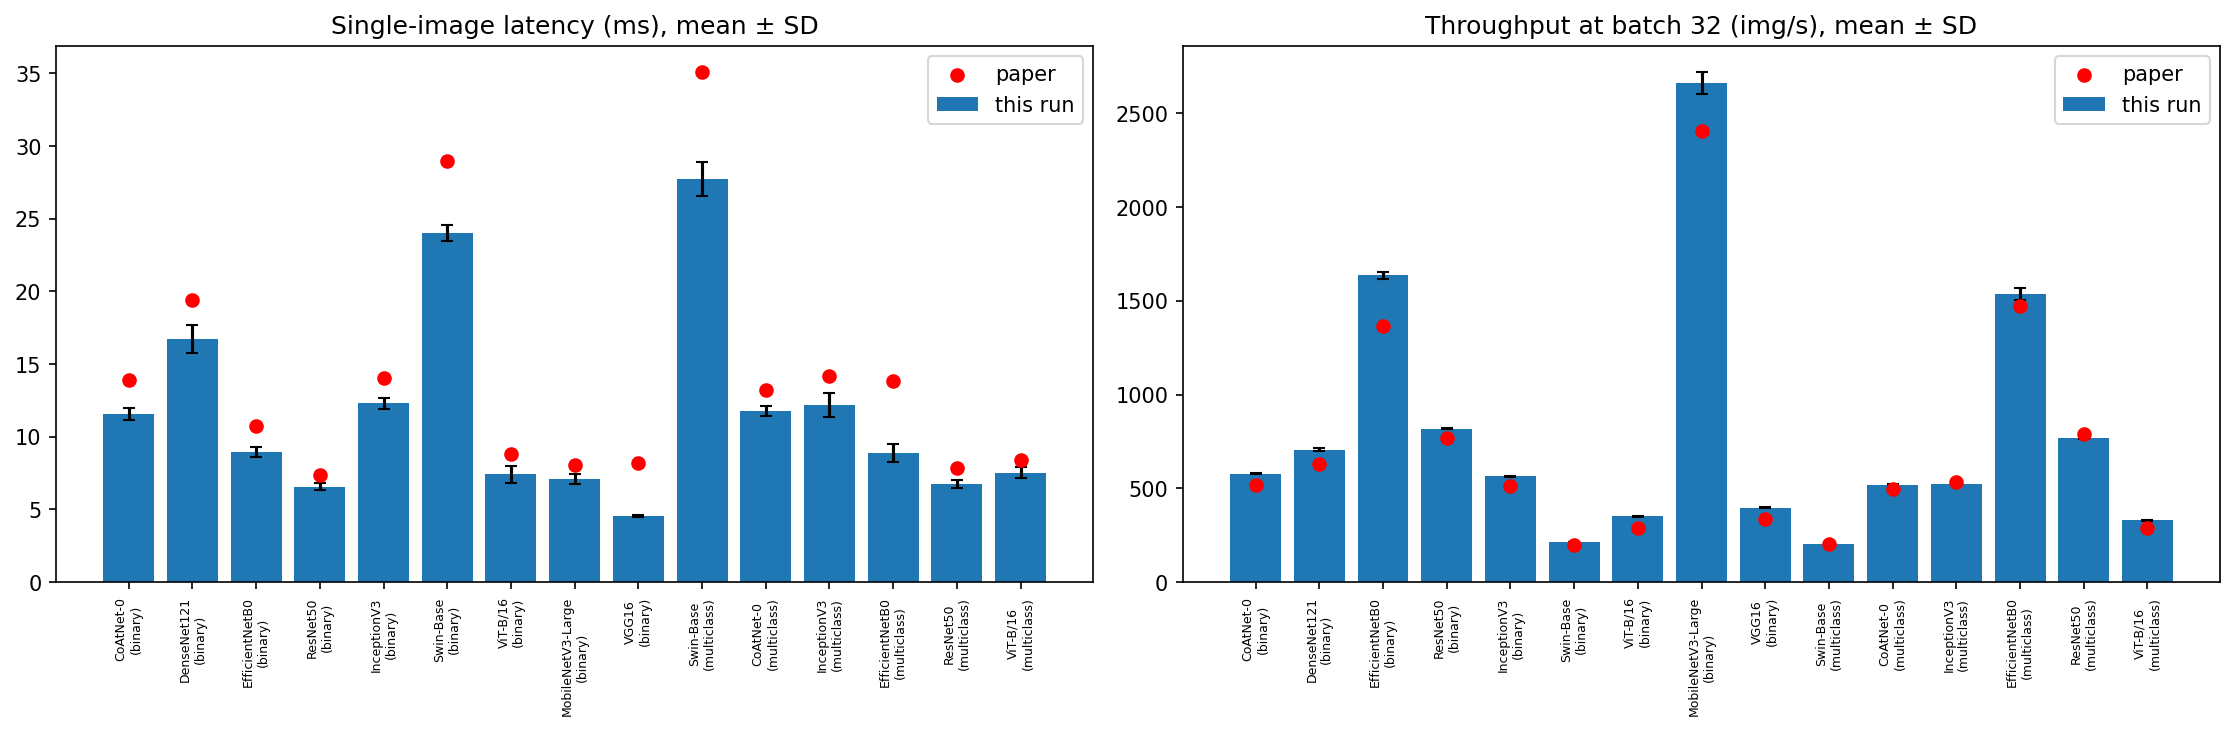
\includegraphics[width=\linewidth]{figures/audit/09_efficiency_with_variance.png}
\caption{Re-measured single-image latency (left) and throughput at batch size 32 (right) for all 15 runs, as the mean $\pm$ within-run standard deviation pooled over three repeats (bars), against the original single-session measurements (dots). The standard deviation between the three repeat means is at most 0.6~ms for latency and 18 images per second for throughput.}
\label{fig:s22}
\end{figure}

\FloatBarrier
\section*{S7. Evaluation figures}

Figures~S9 and S10 show receiver operating characteristic and precision--recall curves for every model on each task, and Figure~S11 the reliability diagrams. Figures~S12 and S13 show the per-class metric summaries and representative test-set predictions of EfficientNetB0, the released checkpoint, and Figure~S14 the complete confusion-matrix panels whose test-split counts are shown in Figures~5--7 of the main text.

\begin{figure}[htbp]
\figurenumber{9}
\centering
\panel{0.32}{figures/supp/binary-detection-coatnet0_roc_pr_curves.png}{CoAtNet-0.}\hfill
\panel{0.32}{figures/supp/binary-detection-densenet121_roc_pr_curves.png}{DenseNet121.}\hfill
\panel{0.32}{figures/supp/binary-detection-efficientnetb0_roc_pr_curves.png}{EfficientNetB0.}
\\[4pt]
\panel{0.32}{figures/supp/binary-detection-resnet50_roc_pr_curves.png}{ResNet50.}\hfill
\panel{0.32}{figures/supp/binary-detection-inceptionv3_roc_pr_curves.png}{InceptionV3.}\hfill
\panel{0.32}{figures/supp/binary-detection-swinbase_roc_pr_curves.png}{Swin-Base.}
\\[4pt]
\panel{0.32}{figures/supp/binary-detection-vit-b16_roc_pr_curves.png}{ViT-B/16.}\hfill
\panel{0.32}{figures/supp/binary-detection-mobilenetv3-large_roc_pr_curves.png}{MobileNetV3-Large.}\hfill
\panel{0.32}{figures/supp/binary-detection-vgg16_roc_pr_curves.png}{VGG16.}
\caption{Receiver operating characteristic and precision--recall curves for all nine models on the binary detection test split. EfficientNetB0 attains an AUC of 0.9998 and an average precision of 0.9998.}
\label{fig:s9}
\end{figure}

\begin{figure}[htbp]
\figurenumber{10}
\centering
\panel{0.32}{figures/supp/classification-swinbase_roc_pr_curves.png}{Swin-Base.}\hfill
\panel{0.32}{figures/supp/classification-coatnet0_roc_pr_curves.png}{CoAtNet-0.}\hfill
\panel{0.32}{figures/supp/classification-inceptionv3_roc_pr_curves.png}{InceptionV3.}
\\[4pt]
\panel{0.32}{figures/supp/classification-efficientnetb0_roc_pr_curves.png}{EfficientNetB0.}\hfill
\panel{0.32}{figures/supp/classification-resnet50_roc_pr_curves.png}{ResNet50.}\hfill
\panel{0.32}{figures/supp/classification-vit-b16_roc_pr_curves.png}{ViT-B/16.}
\caption{One-versus-rest receiver operating characteristic and precision--recall curves for all six models on the multiclass test split. Swin-Base and EfficientNetB0 attain macro-averaged AUCs of 0.9993 and 0.9988.}
\label{fig:s10}
\end{figure}

\begin{figure}[htbp]
\figurenumber{11}
\centering
\panel{0.32}{figures/supp/binary-detection-coatnet0_calibration.png}{Binary, CoAtNet-0.}\hfill
\panel{0.32}{figures/supp/binary-detection-densenet121_calibration.png}{Binary, DenseNet121.}\hfill
\panel{0.32}{figures/supp/binary-detection-efficientnetb0_calibration.png}{Binary, EfficientNetB0.}
\\[4pt]
\panel{0.32}{figures/supp/binary-detection-resnet50_calibration.png}{Binary, ResNet50.}\hfill
\panel{0.32}{figures/supp/binary-detection-inceptionv3_calibration.png}{Binary, InceptionV3.}\hfill
\panel{0.32}{figures/supp/binary-detection-swinbase_calibration.png}{Binary, Swin-Base.}
\\[4pt]
\panel{0.32}{figures/supp/binary-detection-vit-b16_calibration.png}{Binary, ViT-B/16.}\hfill
\panel{0.32}{figures/supp/binary-detection-mobilenetv3-large_calibration.png}{Binary, MobileNetV3-Large.}\hfill
\panel{0.32}{figures/supp/binary-detection-vgg16_calibration.png}{Binary, VGG16.}
\caption{Reliability diagrams for all models on the binary detection test split (continued overleaf for the multiclass task). EfficientNetB0 attains an expected calibration error of 0.0049.}
\label{fig:s11}
\end{figure}

\begin{figure}[htbp]
\ContinuedFloat
\centering
\panel{0.32}{figures/supp/classification-swinbase_calibration.png}{Multiclass, Swin-Base.}\hfill
\panel{0.32}{figures/supp/classification-coatnet0_calibration.png}{Multiclass, CoAtNet-0.}\hfill
\panel{0.32}{figures/supp/classification-inceptionv3_calibration.png}{Multiclass, InceptionV3.}
\\[4pt]
\panel{0.32}{figures/supp/classification-efficientnetb0_calibration.png}{Multiclass, EfficientNetB0.}\hfill
\panel{0.32}{figures/supp/classification-resnet50_calibration.png}{Multiclass, ResNet50.}\hfill
\panel{0.32}{figures/supp/classification-vit-b16_calibration.png}{Multiclass, ViT-B/16.}
\caption{(continued) Reliability diagrams for all models on the multiclass test split. EfficientNetB0 attains an expected calibration error of 0.0112.}
\end{figure}

\begin{figure}[htbp]
\figurenumber{12}
\centering
\panel{0.8}{figures/binary_per_class.png}{Binary detection. The tumour class attains perfect recall, with the residual error confined to precision on that class.}
\\[4pt]
\panel{0.8}{figures/cls_per_class.png}{Multiclass classification, showing meningioma as the weakest of the three classes.}
\caption{Per-class precision, recall, and F1 scores for \textbf{EfficientNetB0} on the test split of each task.}
\label{fig:s12}
\end{figure}

\begin{figure}[htbp]
\figurenumber{13}
\centering
\panel{1}{figures/binary_predictions.png}{Binary detection.}
\\[4pt]
\panel{1}{figures/cls_predictions.png}{Multiclass classification.}
\caption{Representative test-set predictions of \textbf{EfficientNetB0}, with the predicted class and associated probability shown for each image.}
\label{fig:s13}
\end{figure}

\begin{figure}[htbp]
\figurenumber{14}
\centering
\panel{0.49}{figures/binary_confusion.png}{EfficientNetB0, binary detection.}\hfill
\panel{0.49}{figures/binary_resnet_confusion.png}{ResNet50, binary detection.}
\\[4pt]
\panel{0.49}{figures/cls_swin_confusion.png}{Swin-Base, multiclass classification.}\hfill
\panel{0.49}{figures/cls_confusion.png}{EfficientNetB0, multiclass classification.}
\caption{Complete confusion-matrix panels for the validation and held-out test splits, as counts and row-normalised, for the models shown in Figures~5--7 of the main text.}
\label{fig:s14}
\end{figure}

\FloatBarrier
\section*{S8. Gradient-weighted class activation maps}

Figure~S15 gives the complete input, activation, and overlay panels for the most confident correct EfficientNetB0 predictions, whose overlay rows appear in Figure~8 of the main text. Figure~S16 shows the most confident misclassified cases, up to six per model, ranked by the probability assigned to the wrong class; these are the failures in which the model was most assured, not representative ones.

\begin{figure}[htbp]
\figurenumber{15}
\centering
\panel{0.62}{figures/binary_gradcam_correct.png}{Binary detection, showing the two most confident correct predictions per class.}
\\[4pt]
\panel{1}{figures/cls_gradcam_correct.png}{Multiclass classification, showing the two most confident correct predictions for each of glioma, meningioma, and pituitary.}
\caption{Gradient-weighted class activation maps for \textbf{EfficientNetB0} on correctly classified test cases.}
\label{fig:s15}
\end{figure}

\begin{figure}[htbp]
\figurenumber{16}
\centering
\panel{0.48}{figures/binary_gradcam_misclassified.png}{Binary detection. Only three test images were misclassified, so all are shown.}
\\[4pt]
\panel{1}{figures/cls_gradcam_misclassified.png}{Multiclass classification: the six most confident of seventeen errors.}
\caption{Gradient-weighted class activation maps for \textbf{EfficientNetB0} on misclassified test cases, ranked by confidence in the wrong class.}
\label{fig:s16}
\end{figure}

Figures~S23 to S25 quantify the EfficientNetB0 maps on the full test split of each task, using the released checkpoints, which reproduce the stored test predictions exactly. Figure~S23 shows the head mask used, Figure~S24 the share of Grad-CAM energy falling outside it, and Figure~S25 an inference-only masking test. The remaining checkpoints, including Swin-Base, were not available to this analysis.

\begin{figure}[htbp]
\figurenumber{23}
\centering
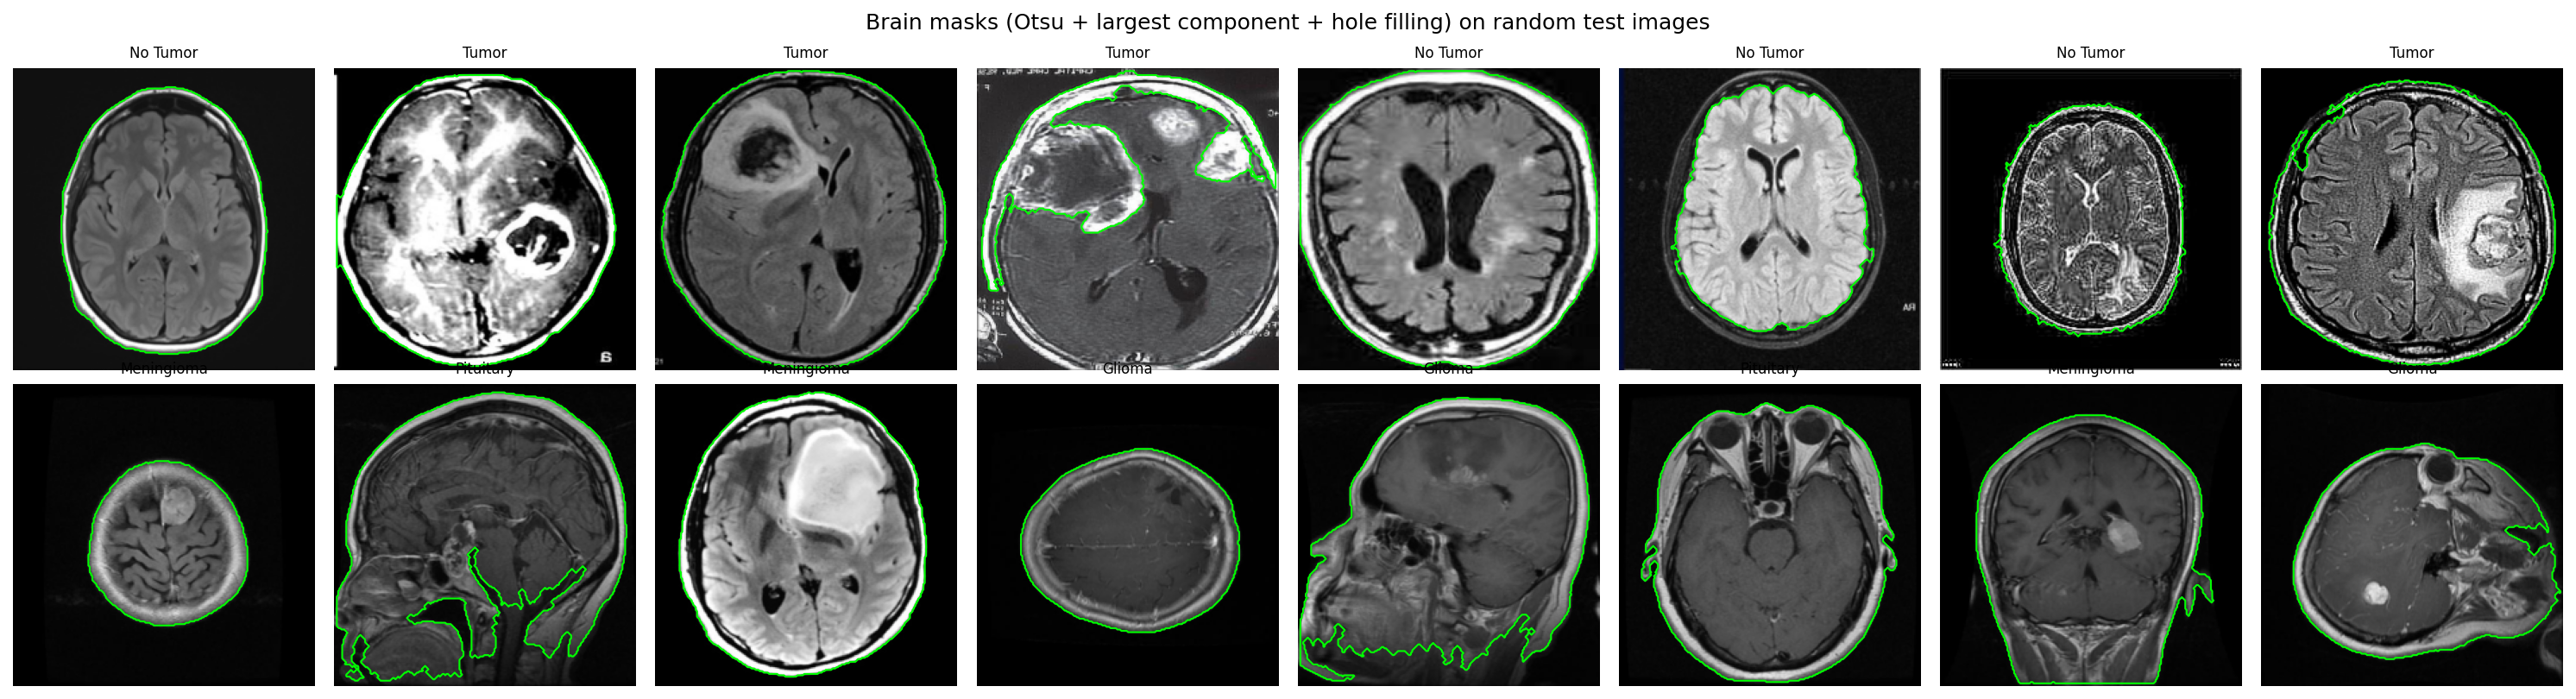
\includegraphics[width=\linewidth]{figures/audit/06_brain_mask_quality_check.png}
\caption{Head masks (green contours) on random binary (top) and multiclass (bottom) test images, computed by Otsu thresholding, a small morphological closing, selection of the largest connected component, and hole filling. The mask covers brain and skull, so energy outside it lies on background, borders, and framing. On sagittal slices it also includes the neck, and on some heavily processed images it misses part of the head.}
\label{fig:s23}
\end{figure}

\begin{figure}[htbp]
\figurenumber{24}
\centering
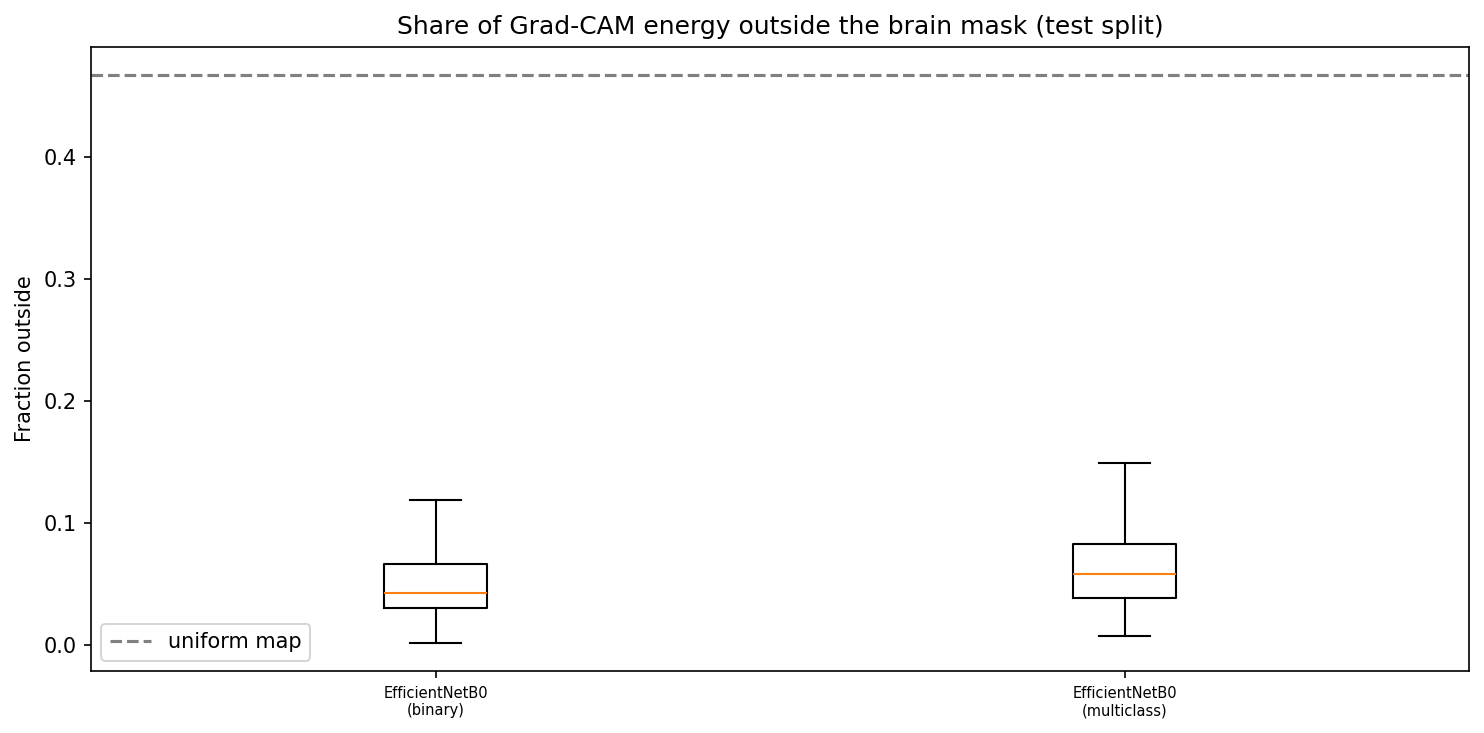
\includegraphics[width=0.85\linewidth]{figures/audit/07_gradcam_outside_brain.png}
\caption{Share of \textbf{EfficientNetB0} Grad-CAM energy falling outside the head mask on the test split, per task. Mean $\pm$ standard deviation per class: tumour-negative $0.068\pm 0.118$ and tumour-positive $0.077\pm 0.118$; glioma $0.040\pm 0.020$, meningioma $0.090\pm 0.044$, and pituitary $0.092\pm 0.110$. A map spread evenly over the image would place 0.39 to 0.53 of its energy outside the mask, depending on class (dashed line, mean).}
\label{fig:s24}
\end{figure}

\begin{figure}[htbp]
\figurenumber{25}
\centering
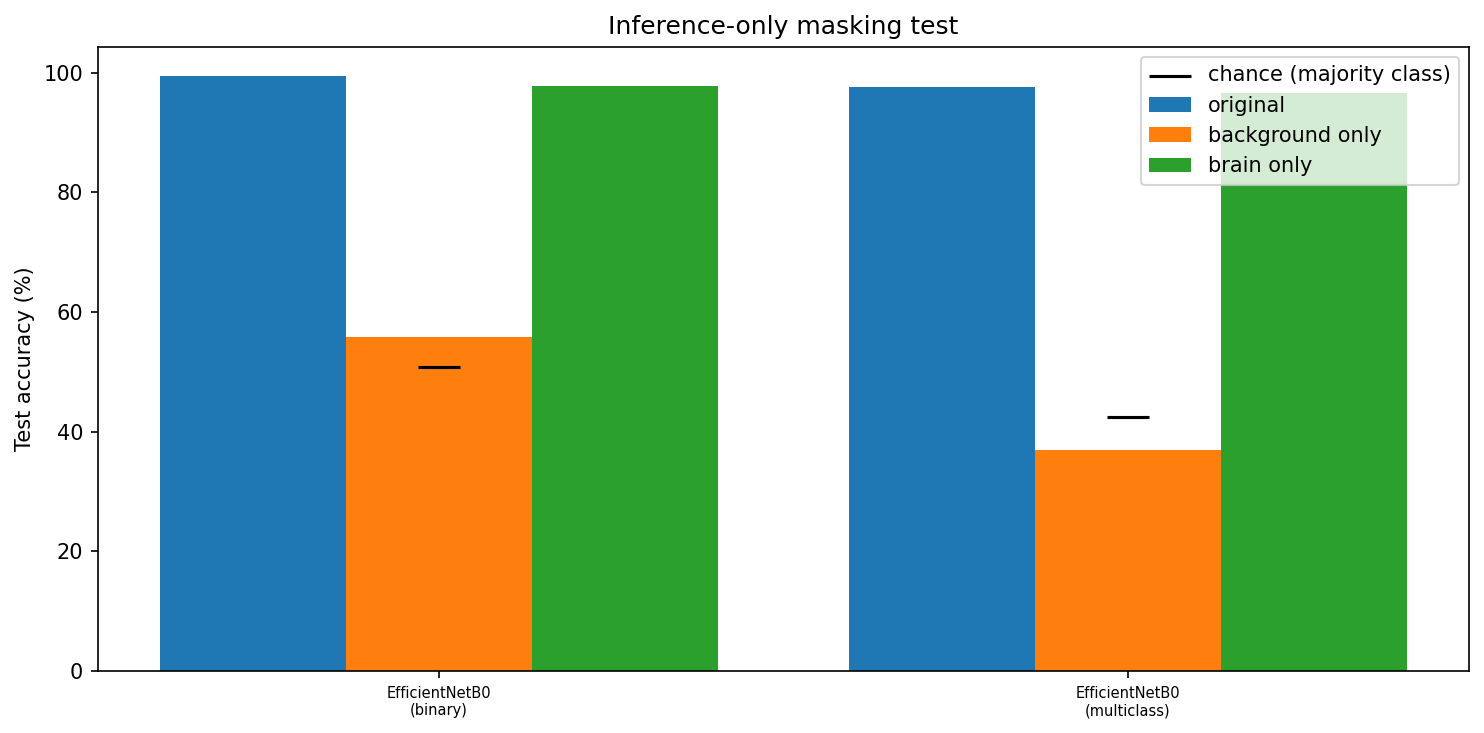
\includegraphics[width=0.85\linewidth]{figures/audit/08_masking_test.png}
\caption{Inference-only masking test for \textbf{EfficientNetB0}: test accuracy on the original images, on background-only images with the head region set to zero, and on head-only images with the background set to zero, against the majority-class rate. Background-only accuracy is 55.74\% against 50.82\% for binary detection and 36.97\% against 42.49\% for subtype classification; head-only accuracy is 97.75\% and 96.60\%. A fall to chance does not rule out a shortcut, because background-only images lie outside the training distribution.}
\label{fig:s25}
\end{figure}

\end{document}
